%; whizzy chapter
% -initex iniptex -latex platex -format platex -bibtex jbibtex -fmt fmt
% $B0J>e(B whizzytex $B$r;HMQ$9$k>l9g$N@_Dj!#(B

%     Tokyo Debian Meeting resources
%     Copyright (C) 2010 Junichi Uekawa

%     This program is free software; you can redistribute it and/or modify
%     it under the terms of the GNU General Public License as published by
%     the Free Software Foundation; either version 2 of the License, or
%     (at your option) any later version.

%     This program is distributed in the hope that it will be useful,
%     but WITHOUT ANY WARRANTY; without even the implied warranty of
%     MERCHANTABILITY or FITNESS FOR A PARTICULAR PURPOSE.  See the
%     GNU General Public License for more details.

%     You should have received a copy of the GNU General Public License
%     along with this program; if not, write to the Free Software
%     Foundation, Inc., 51 Franklin St, Fifth Floor, Boston, MA  02110-1301 USA

%  preview (shell-command (concat "evince " (replace-regexp-in-string "tex$" "pdf"(buffer-file-name)) "&"))
% $B2hA|%U%!%$%k$r=hM}$9$k$?$a$K$O(Bebb$B$rMxMQ$7$F(Bboundingbox$B$r:n@.!#(B
%(shell-command "cd image201011; ebb *.jpg")

%%$B$3$3$+$i%X%C%@3+;O!#(B

\documentclass[mingoth,a4paper]{jsarticle}
\usepackage{monthlyreport}
\usepackage{wrapfig}

% $BF|IU$rDj5A$9$k!"Kh7nJQ$o$j$^$9!#(B
\newcommand{\debmtgyear}{2010}
\newcommand{\debmtgmonth}{11}
\newcommand{\debmtgdate}{20}
% (+ (* (- 2010 2005) 12) 10) started from zero
\newcommand{\debmtgnumber}{70}

\begin{document}

\begin{titlepage}
\thispagestyle{empty}
% $B%?%$%H%k%Z!<%8(B:$BJT=8I,MW$JItJ,$O:G=i$N%^%/%m$KHt$P$9$3$H(B

\vspace*{-2cm}
$BBh(B\debmtgnumber{}$B2s(B $BEl5~%(%j%"(B Debian $BJY6/2q;qNA(B\\
\hspace*{-2cm}
\includegraphics[width=210mm]{image201003/debsen.eps}\\
\hfill{}\debmtgyear{}$BG/(B\debmtgmonth{}$B7n(B\debmtgdate{}$BF|(B

% $B$3$3$O%"%C%W%G!<%H$9$k$3$H(B
\rotatebox{10}{\fontsize{32}{32} {\gt $BFC=8(B: $B26$N%U%!%$%k%7%9%F%`$OG.$$$<!*(B}}

\vspace*{-2cm}
\hfill{}
\includegraphics[height=6cm]{image200502/openlogo-nd.eps}
\end{titlepage}

\dancersection{Introduction}{$B>e@n(B $B=c0l(B}

\begin{multicols}{2}
 

 $B:#7n$N(BDebian$BJY6/2q$X$h$&$3$=!#$3$l$+$i(BDebian$B$N@$3&$K$"$7$rF'$_F~$l$k$H(B
 $B$$$&J}$b!"$9$G$K$I$C$W$j$H$D$+$C$F$$$k$H$$$&J}$b!"7n$K0l2s(BDebian$B$K$D$$(B
 $B$F8l$j$^$;$s$+!)(B

 Debian$BJY6/2q$NL\E*$O2<5-$G$9!#(B

 \begin{itemize}
 \item \underline{Debian Developer} ($B3+H/<T(B)$B$N0i@.!#(B
 \item $BF|K\8l$G$N!V(B\underline{$B3+H/$K4X$9$k>pJs(B}$B!W$r@0M}$7$F$^$H$a!"%"%C%W%G!<%H$9$k!#(B
 \item \underline{$B>l(B}$B$NDs6!!#(B
 \begin{itemize}
  \item $BIaCJ$P$i$P$i$J>l=j$K$$$k?M!9$,(B face-to-face $B$G=P2q$($k>l$rDs6!(B
	$B$9$k!#(B
  \item Debian $B$N$?$a$K$J$k$3$H$r8l$k>l$rDs6!$9$k!#(B
  \item Debian$B$K$D$$$F8l$k>l$rDs6!$9$k!#(B
 \end{itemize}
 \end{itemize}		

 Debian$B$NJY6/2q$H$$$&$3$H$G5f6KE*$K$O;22C<TA40w$,(BDebian Package$B$r$,$j$,$j(B
 $B$H:n$k%9!<%Q!<%O%C%+!<$K$J$C$?;Q$rLQA[$7$F$$$^$9!#>pJs$N6&M-!&3hMQ$rDL$7(B
 $B$F(B Debian$B$N:#8e$NG=F0E*$JE83+$X$NEZBf$H$7$F!"!V>l!W$H$7$F$N6u4V$rDs6!$9(B
 $B$k$N$,L\E*$G$9!#(B

\end{multicols}

\newpage

\begin{minipage}[b]{0.2\hsize}
 \definecolor{titleback}{gray}{0.9}
 \colorbox{titleback}{\rotatebox{90}{\fontsize{80}{80} {\gt $B%G%S%"%sJY6/2q(B} }}
\end{minipage}
\begin{minipage}[b]{0.8\hsize}
\hrule
\vspace{2mm}
\hrule
\begin{multicols}{2}
\tableofcontents
\end{multicols}
\vspace{2mm}
\hrule
\end{minipage}

\dancersection{$B;vA02]Bj(B}{$B>e@n(B $B=c0l(B}

$B:#2s$N;vA02]Bj$O0J2<$G$9(B:
\begin{itemize}
 \item $BF|>oE*$K3hMQ$7$F$$$k%U%!%$%k%7%9%F%`@_Dj$K$D$$$F>R2p$9$k!#(B($BNc!"(BLVM, ext3, jffs, ...)
\end{itemize}
$B$3$N2]Bj$KBP$7$FDs=P$$$?$@$$$?FbMF$O0J2<$G$9!#(B

 \begin{prework}{ ����(yy\_y\_ja\_jp) }
���ޤ���������ǤϤʤ��Ǥ���... �긵�Υ�åץȥåפǤ� /boot �ˤ� ext2
 ����¾�ˤ� ext3���Ƕ�ȤäƤ���ǥ����ȥåפǤ� /boot �ˤ� ext3 ����¾
 �ˤ� LVM ��� ext4 ��ȤäƤ��ޤ���
\end{prework}

\begin{prework}{ �����ϥ� }
�ǥե���Ȥ�ext3����
�����ǥե���ȤΤޤޡ�
(NTFS���VM���᡼�����ext3�⤢�뤱��)
\end{prework}

\begin{prework}{ yos.takahashi }
ext3/4���˻ȤäƤޤ���ext3�Υǡ�������١����ˤĤ�������Linux2011ǯ1���˼�ɮ���ޤ�����
\end{prework}

\begin{prework}{ MATOHARA }
����inode �ϳ���������Ƥ���inode ��ưŪ�˳�����Ƥ���XFS �����򤹤뤳
 �Ȥ�¿���Ǥ���NILFS �Ͼ�����Ƥߤ��ΤǤ�����mount ���˰ʲ��Τ褦�ʥ��
 ���������ФƤޤ��ݤ��ʤȻפ��ޤ�����
\begin{commandline}
$ sudo mount /dev/sdb1 /mnt
mount.nilfs2: WARNING! - The NILFS on-disk format may change at any time.
mount.nilfs2: WARNING! - Do not place critical data on a NILFS filesystem. 
\end{commandline}
����¾NotePC �Ǥ�dm-crypt �ξ�˥ե����륷���ƥ���֤��ưŹ沽�����ꡢ
 eCryptfs �ǰŹ沽�����ꤷ�Ƥ��ޤ����񤭹��߻���CPU �򤫤ʤ���񤷤ޤ��ġ�
\end{prework}

\begin{prework}{ ��ޤ� }
��ext2-$>$reiserfs-$>$jfs-$>$xfs-$>$reiserfs-$>$ext3�ȻȤäƤ��ޤ�����

����:
\begin{itemize}
 \item reiserfs: ���ե������¿���ե�����Υ������������ӥ��Ӥ��Ƥ��ɤ���
       �����������դȤ����ⵤ�������θ�μ�žȬ�ݥ����ɤˡ�����
 \item jfs: ����v1.0��̾��ä�IBM���ꥨ�ʥ��������ˤ�xfs��ƨ��
 \item xfs: fsck==true�˴�ư����������ǯ�Ȥä���ΤΥޥ�����Ĵ����0byte
       �ե��������������Ѥ���줺ƨ����
\end{itemize}
������reiser4��Ķ���Ԥ��뤦���ˤ��줬�����ʤäơ����ext3�˸��경��htree�����ä������⤦Ŵ�Ĥʤ鲿�Ǥ⤤���Ǥ��������Ȥ����Ĥ�nilfs�ʤɤ˼��Ф��Ƥ��ޤ���ext3�������noatime���٤Ǥ����������aufs���碌�Ƽ�ʬ���Ȥ��Ȥ� *strap �Ķ��򥯥����˥󥰤��Ƥ��ޤ����¸����ƥ��Ȥ������Ǥ�����Ǥ���USB�����ư�Ǥ�ͭ�ѡ�

���LVM�ǤϤʤ�MD��Ȥäƾ�Ĺ���ܥХå����åפ򤷤Ƥ��ޤ���
 MD(sda,sdb,sdc)�ǹ��ۤ����̾��MD(����)�Dz�ư���Хå����åפλ���
 attach/detach�򤹤롣�֥��å���٥�ʤΤǥꥫ�Х��FSǤ���Ǥ��������̤�
 �������¾����ˡ���ʤ�������
\end{prework}

\begin{prework}{ henrich }
�ȤäƤ���֤�NTFS��Ĺ���󤸤�ʤ��Ǥ����͡����졣
�����Ρ����Ѥο������ǥ�������ext4�ǥե����ޥåȤ��ޤ����������㤤��Ƚ��ʤ��Ȥ����������Ƥ��ޤ���
\end{prework}

\begin{prework}{ emasaka }
�Ĥ뤷��FS��ȤäƤޤ�
\end{prework}

\begin{prework}{ �ܾ� }
ext3����Ѥ��Ƥ��ޤ����ä��Ѥ�ä����ȤϤ��Ƥ��ޤ���
FS����ʤ��Ǥ������Ƕ�Lenny��2TB��HDD��Ȥä���parted�äƤλȤ��ƶä��ޤ�����
\end{prework}

\begin{prework}{ ����@������ }
���������Ū�˳��Ѥ��Ƥ���ե����륷���ƥ��ReiserFS�Ǥ���
�Ż��ǻȤäƤ�Ķ���ext3�Ǥ�����ext3���Ÿ������ǥ��㡼�ʥ뤬
����Ʋ��Ǥ������ηи��ʸŤ������ͥ�Ǥ���...�ˤ����ꡢ
���ޤ꿮�Ѥ��Ƥ��ޤ���
�����ReiserFS�Ķ��ǤϤ���ޤǤνꤤ���ʤ��Ÿ����ڤä��ꡢ
�Ƥ�HDD�����줫�����ꤷ�Ƥ��ﳲ����ä��и���̵���Τǡ�
��³Ū�˻ȤäƤ��ޤ���
��ǯ����ReiserFS�Υᥤ��ȯ��(Hans Reiser)�����ᤵ��Ƥ��ޤ������ƥʥ󥹤��ۤ��Ƥ��ޤ�����
�����������θ��ReiserFS��¾�γ�ȯ�Ԥˤ���³�����ݼ餵��Ƥ���Τǡ��¿����ޤ�����
\end{prework}

\begin{prework}{ nozzy123nozzy }
\begin{enumerate}
 \item LVM�ˤĤ��Ƥϡ�CentOS5.5��Ƴ�������Τ��Τޤޤ����Ѥ��Ƥޤ�����
       ���������ƥब��äƤ���Volume̾�ϥǥե���Ȥ�����ȡʼºݤˤ�
       kickstart�ˤơˤ��ѹ����ƻȤäƤޤ����ʾ㳲���Υ���١����˺��뤿
       ���
\item ext3�ˤĤ��Ƥϡ�debian-sid�����Τޤ޻��ꤷ�Ƥ����Τ򤽤Τޤ޻Ȥ�
      �Ƥ����ꤷ�ޤ���relatime, noatime ���餤�Ͼ����ɲä��Ƥߤ����ʡ���
      �ϻפäƤޤ���
\end{enumerate}
\end{prework}

\begin{prework}{ �ޤ��������ؤ� }
\begin{itemize}
 \item Debian�Ǥ��ä˶Ťä����Ȥ�����ext3��ȤäƤޤ������ۥޥ����qcow2
       ���᡼���ǥ��������ѻ��ʳ��ϡ�LVM�ϻȤäƤޤ���
 \item �����ǰ����ü�ʤΤϡ��������DHCP�������Ѥ�Armadillo-J�ǻȤäƤ�
       ��JFFS�Ǥ����ǥե���ȤΥե����०�����Ǥϥ�֡��Ȥ�����������
       �ƽ��������Ƥ��ޤ��Τǡ�RAM�ΰ�˽񤭤��ߡ��Ÿ��ڤäƤ�ä��ʤ�
       ���������Ǥ���Debian��udhcp�Υ������ѥå���������ӥ�ɤ��ƻȤäƤޤ���
       \footnote{\url{http://d.hatena.ne.jp/mkouhei/20080601/1212330630}}
 \item ��Debian���ߤǡ���ʬ����ǰ��֥ۥåȤʤΤ�palm webOS�Ǥ��������Ubuntu��
       �������ޥ���������Τ餷���ΤǤ�����/etc/mtab�򸫤��35�Ԥ⤢�ꡢ
       ���ʤ����֤ʹ����Ǥ��͡�
\end{itemize}
\end{prework}

\dancersection{$B:G6a$N(BDebian$B4XO"$N%_!<%F%#%s%0Js9p(B}{$B$^$($@$3$&$X$$(B}
\subsection{$BEl5~%(%j%"(BDebian$BJY6/2q(B69$B2sL\Js9p(B}

$B5W!9$NDL>o$I$*$j$N(BDebian$BJY6/2q$O(B10/16$B$K!">l=j$OBg?9$N%K%U%F%#$5$s$N%;%_(B
$B%J!<%k!<%`$r$*<Z$j$7$F3+:E$7$^$7$?!#JY6/2q$N%5%$%H$G$OBh(B69$B2s$H$J$C$F$$$^(B
$B$9$,!"(B8$B7n$O3+:E$7$F$$$J$$$N$G:#2s$O@53N$K$O(B68$B2s$G$9(B*1$B!#;*FI$s$G$^$9!#(B
$B$,!"(B68$B2s$O7gHV$H$7$^$7$?!#(B

\subsubsection{$B3+:EFbMF(B}
$B:#2s$O:G6a$N%$%Y%s%H!"$H$/$K(BLinuxCon Japan 2010$B$H(BDebconf10$B$N;22CJs9p$N$"(B
$B$H!";vA02]Bj$N!V26$N(BDebian$B$J0lF|!W$r;22C<TA40w$K<+8J>R2p$r7s$M$FH/I=$7$F(B
$BLc$$!"F|K\$G$N(BMini Debconf$B3+:E$K8~$1$F$N%V%l%9%H$r9T$$$^$7$?!#:#2s=i;22C(B
$B$N(Bhattorin$B$5$s$H(Btan$B$5$s$,<!2s%M%?$rH/I=$7$F$/$l$k$3$H$K$J$C$?$3$H!"(BMini
Conf$B$K8~$1$F$N%G%#%9%+%C%7%g%s$O<!2s0J9_$bB3$1$F$$$/$3$H$K$J$j$^$7$?!#(B

\subsubsection{$B;22C<T(B}
$B;22C<T(B($B7I>NN,(B)$B$O!"(Btai$B!"F|HfLn!"$"$i$-!"(Bhattorin$B!"5HLn!"%-%?%O%i!">.<<!"(B
$B;3K\!"NkLZ!"$"$1$I!"$d$^$M!">e@n!"$^$($@$N7W(B13$B?M$G$7$?!#(B

$B%K%U%F%#$5$s$"$j$,$H$&!*(B
$B%K%U%F%#$5$s$K$O2q>l$r$*<Z$j$7$?$@$1$G$J$/!"JY6/2q$N:G8e$KL5Cc$V$j$7$F$b(B
$B$-$A$s$H%3%a%s%H$bD:$-!"@?$K$"$j$,$H$&$4$6$$$^$7$?!#(B

\subsubsection{$B1c2q(B}
$B1c2q$O$7$c$V$7$c$V29Ln:Z(B $BBg?9E9$G9T$$$^$7$?!#(B

% (query-replace-regexp "<.*?>" "")
% (query-replace-regexp "^[	 ]\+" "")

%-------------------------------------------------------------------------------
\dancersection{ext4 $B%U%!%$%k%7%9%F%`$r(BDebian$B$G3hMQ$7$F$_$k(B}{$B>e@n(B $B=c0l(B}
%-------------------------------------------------------------------------------
\index{ext4}

ext4 $B%U%!%$%k%7%9%F%`$O(B Linux $B$G9-$/;H$o$l$F$$$k(B ext3 $B$N8e7Q%U%!%$%k%7%9(B
$B%F%`$H$7$FEP>l$7$?%U%!%$%k%7%9%F%`$G$9!#FCD'$H$7$F$O!"(Bext3 $B$HF1$8$/%8%c!<(B
$B%J%j%s%05!G=$r$b$A!"%G!<%?NN0h$r%V%m%C%/C10L$G$O$J$/%(%/%9%F%s%H(B($B0lO"$NNN(B
$B0h(B)$B$G3NJ]$7$F$$$k$3$H!#(B32$B%S%C%H$+$i(B48$B%S%C%H$K$J$C$?$N$G!"%U%!%$%k%7%9%F%`(B
$B%5%$%:$,(Bext3 $B$N@)8B$r1[$($F$$$k!#(Batime$B$J$I$,IC$h$j:Y$+$$;~4V$G$o$+$k$h$&(B
$B$K$J$k!"$J$I$G$9!#(B\cite{ext42007,ext42008}

\subsection{ext4 $B%U%!%$%k%7%9%F%`$r:n$C$F$_$k(B}

$B$=$l$G$O!"(Bext4$B%U%!%$%k%7%9%F%`$r:n$C$F$_$^$7$g$&!#<B$ODL>o$N(Bext3$B%U%!%$%k(B
$B%7%9%F%`$r$=$N$^$^(Bext4$B$H$7$F%^%&%s%H$9$k$3$H$b$G$-$k$h$&$G$9!#$=$&$9$k$H=y!9$K(B
$B%U%!%$%k$,=q$-49$($k$?$S$K(Bextent$B%Y!<%9$K$J$C$?$j$9$k$h$&$G$9!#(B
$B$?$@!"%U%!%$%k%7%9%F%`A4BN$N%Q%i%a!<%?$,(Bext4$BMQ$G$O$J$$$N$G!"%U%!%$%k%7%9(B
$B%F%`$r$$$A$+$i:n@.$9$k$N$,$h$$$G$7$g$&!#(B

$B%"%m%1!<%?$N%"%k%4%j%:%`$b2~A1$5$l$F$$$k$N$G>.$5$J%U%!%$%k$N%"%m%1!<%7%g(B
$B%s$b2~A1$7$F$$$k$h$&$G$9$N$G!"4{B8$N%U%!%$%k%7%9%F%`$NFbMF$r%P%C%/%"%C%W(B
$B$7$F%j%9%H%"$9$k$N$,$h$$$N$G$O$J$$$G$7$g$&$+!#(B

ext4 $B$r;H$&$K$O==J,?7$7$$(B e2fsprogs $B$H==J,$"$?$i$7$$(BLinux Kernel $B$,$"$l$P(B
$B$h$$$G$9!#(BDebian 5.0 (lenny) $B$N;~E@$GI,MW$J%Q%C%1!<%8$O$=$m$C$F$$$k$h$&$G$9!#(B

\begin{commandline}
 $ sudo lvcreate -L 1G -n lvext4 vghoge
  Logical volume "lvext4" created
 $ sudo mount /dev/vghoge/lvext4 /mnt/
 $ mount -v 
 /dev/mapper/vghoge-lvext4 on /mnt type ext4 (rw)
 $ df -h /mnt/
 Filesystem          $B%5%$%:(B  $B;HMQ(B  $B;D$j(B $B;HMQ(B% $B%^%&%s%H0LCV(B
 /dev/mapper/vghoge-lvext4
                     1008M   34M  924M   4% /mnt
 $ df -T /mnt/ 
 Filesystem    Type   1K-$B%V%m%C%/(B    $B;HMQ(B   $B;HMQ2D(B $B;HMQ(B% $B%^%&%s%H0LCV(B
 /dev/mapper/vghoge-lvext4
              ext4     1032088     34052    945608   4% /mnt
 $ df -i /mnt/
 Filesystem            I$B%N!<%I(B  I$B;HMQ(B   I$B;D$j(B I$B;HMQ(B% $B%^%&%s%H0LCV(B
 /dev/mapper/vghoge-lvext4
                       65536      11   65525    1% /mnt
\end{commandline}

\begin{thebibliography}{0}
 \bibitem{ext42007} A. Mathur, M. Cao, S. Bhattacharya, A. Dilger, A. Tomas, and
 L. Vivier. "The new ext4 filesystem: current status and future plans,"
 Linux Symposium. 2007

 \bibitem{ext42008}  A. Kumar K. V., M. Cao, J. R. Santos, and A. Dilger. "Ext4 block and inode allocator improvements," Linux Symposium, Vol 1. 2008.

\end{thebibliography}

%-------------------------------------------------------------------------------
\dancersection{NILFS$B$r(BDebian$B$G3hMQ$7$F$_$k(B}{$B;3ED(B $BBY;q(B}
%-------------------------------------------------------------------------------
\index{NILFS}

\subsection{NILFS$B$C$F$I$s$J%U%!%$%k%7%9%F%`(B?}
\subsection{$B%$%s%9%H!<%kJ}K!(B}

Debian$B$G%$%s%9%H!<%k$9$kJ}K!(B

\subsection{$B%^%&%s%H!&(Bfsck}


\subsection{$B%P%C%/%"%C%WMQ$N%U%!%$%k%7%9%F%`$H$7$F;H$C$F$_$k(B}

%-------------------------------------------------------------------------------
\dancersection{Btrfs$B$r(BDebian$B$G3hMQ$7$F$_$k(B}{$BNkLZ(B $B?rJ8(B}
%-------------------------------------------------------------------------------
\index{Btrfs}

\subsection{Btrfs$B$C$F$I$s$J%U%!%$%k%7%9%F%`(B?}
Btrfs $B$O!"(BLinux kernel $B$N(B 2.6.29 $B$+$i(B kernel $B$N%j%j!<%9$K$b4^$^$l$k$h$&$K$J$C$?!"?7$7$$%3%T!<%*%s%i%$%H7A<0$N%U%!%$%k%7%9%F%`$G$"$j!"%U%)!<%k%H%H%l%i%s%H$d=$I|5!G=!"MF0W$J4IM}5!G=$J$I$,Hw$o$C$F$$$^$9!#(BZFS $B$N1F6A$r<u$1$F$$$k$H8@$o$l$F$*$j!"(BOracle $B$N(B Chris Mason $B$K$h$j(B GPL $B$G3+H/$,$9$9$a$i$l$F$$$^$9!#(B
$B8=:_$O$^$@3+H/Cf$N>uBV$K$"$j$^$9!#(B

$B$J$*!":#2s$O(B Squeeze/Sid $B$r;HMQ$7$F2r@b$7$^$9$,!"(BSqueeze/Sid $B$N(B README\footnote{/usr/share/doc/btrfs-tools/README.Debian} $B$K$*$$$F$b!"$^$@8=;~E@$G$O%Y%s%A%^!<%/$H%l%S%e!<0J30$K;HMQ$9$k$J$H$NCm0U=q$-$,$"$j$^$7$?!#(B
\begin{commandline}
btrfs-tools for Debian
----------------------

WARNING: Btrfs is under heavy development, and is not suitable for any uses
other than benchmarking and review.

 -- Daniel Baumann <daniel@debian.org>  Sun, 29 Jul 2007 12:19:00 +0200
\end{commandline}

\subsection{Debian$B$G%$%s%9%H!<%k$9$kJ}K!(B}
Debian $B$G(B Btrfs $B$r;HMQ$9$k<j=g$O!"(Bbtrfs-tools$B%Q%C%1!<%8$r%$%s%9%H!<%k$9$k$@$1$K$J$j$^$9!#(B
\begin{commandline}
$ sudo apt-get install btrfs-tools
\end{commandline}

\subsection{$B%U%)!<%^%C%H!&%^%&%s%H!&(Bbtrfsck}

$B%U%)!<%^%C%H$O(B\texttt{mkfs.btrfs}$B$G9T$($^$9!#(B
\begin{commandline}
# mkfs.btrfs /dev/sda

WARNING! - Btrfs Btrfs v0.19 IS EXPERIMENTAL
WARNING! - see http://btrfs.wiki.kernel.org before using

fs created label (null) on /dev/sda
        nodesize 4096 leafsize 4096 sectorsize 4096 size 500.00MB
Btrfs Btrfs v0.19
\end{commandline}

$B%^%&%s%H$bDL>oDL$j!"(B\texttt{mount}$B$r;HMQ$G$-$^$9!#(B
\begin{commandline}
# mkdir /mnt/btrfs1
# mount /dev/sda /mnt/btrfs1
# df -T
Filesystem    Type   1K-blocks      Used Available Use% Mounted on
/dev/sde1     ext3    19272572   2833388  15460192  16% /
tmpfs        tmpfs      517260         0    517260   0% /lib/init/rw
udev         tmpfs      512936       100    512836   1% /dev
tmpfs        tmpfs      517260         0    517260   0% /dev/shm
/dev/sda     btrfs      512000    205092    306908  41% /mnt/btrfs1
\end{commandline}

$B$3$3$G;n$7$K%U%!%$%k$r%3%T!<$7$F$_$k$H!"<!$N$h$&$K%3%T!<%*%s%i%$%H$N$*$+$2$G9bB.$J%3%T!<$,$5$l$F$$$k$3$H$,$o$+$j$^$9!#(B
\begin{commandline}
# ls -al /mnt/btrfs1/
total 102408
dr-xr-xr-x 1 root root         8 Nov 17 04:14 .
drwxr-xr-x 3 root root      4096 Nov 17 04:01 ..
-rw-r--r-- 1 root root 104857600 Nov 17 04:03 data
# time cp /mnt/btrfs1/data  /mnt/btrfs1/data-copy

real    0m0.731s
user    0m0.000s
sys     0m0.556s
# ls -al /mnt/btrfs1/
total 116584
dr-xr-xr-x 1 root root        26 Nov 17 04:14 .
drwxr-xr-x 3 root root      4096 Nov 17 04:01 ..
-rw-r--r-- 1 root root 104857600 Nov 17 04:03 data
-rw-r--r-- 1 root root 104857600 Nov 17 04:14 data-copy
\end{commandline}

$B%I%-%e%a%s%H$K$O(B\texttt{fsck}$B$O$^$@40A4$K$O<BAu$5$l$F$*$i$:!"%"%s%^%&%s%H$5$l$?>uBV$G(BFS$B%(%/%9%F%s%H%D%j!<$N%A%'%C%/$N$_$,<BAu$5$l$F$$$k!"$H5-:\$5$l$F$$$^$7$?$,!"<B:]$K<B9T$7$?$H$3$m$G$O%^%&%s%H>uBV$G$"$C$F$b<B9T$G$-$^$7$?!#(B
$B$J$*!"!V(B\texttt{-a}$B!W%*%W%7%g%s$,<BAu$5$l$F$$$J$$$?$a8=;~E@$G$O(B\texttt{fsck.btrfs}$B$X$N%7%s%\%j%C%/%j%s%/$OB8:_$;$:!"(B\texttt{btrfsck}$B$rD>@\<B9T$9$kI,MW$,$"$j$^$9!#(B
\begin{commandline}
# btrfsck /dev/sda
found 210018304 bytes used err is 0
total csum bytes: 204800
total tree bytes: 303104
total fs tree bytes: 8192
btree space waste bytes: 74736
file data blocks allocated: 209715200
 referenced 209715200
Btrfs Btrfs v0.19
\end{commandline}

\subsection{$BJ#?t$N%G%#%9%/$r;HMQ$7$F$_$k(B}
Btrfs$B$G$OJ#?t$N%G%#%9%/$NB+$M$F;HMQ$9$k$3$H$b$G$-$^$9!#$3$3$G$O@h$[$I:n@.$7$?(B /dev/sda $B$K(B /dev/sdb $B$rDI2C$7$F$_$^$9!#(B\texttt{btrfs device add}$B$G4JC1$KDI2C$G$-$^$9!#(B\texttt{df}$B$GDI2C$7$?J,$NMFNL$,A}$($F$$$k$3$H$,3NG'$G$-$^$9!#(B
\begin{commandline}
# df
Filesystem           1K-blocks      Used Available Use% Mounted on
/dev/sde1             19272572   3414148  14879432  19% /
tmpfs                   517260         0    517260   0% /lib/init/rw
udev                    512936       100    512836   1% /dev
tmpfs                   517260         0    517260   0% /dev/shm
/dev/sda                512000        28    511972   1% /mnt/btrfs1
# btrfs device add /dev/sdb /mnt/btrfs1/
# df
Filesystem           1K-blocks      Used Available Use% Mounted on
/dev/sde1             19272572   3414148  14879432  19% /
tmpfs                   517260         0    517260   0% /lib/init/rw
udev                    512936       100    512836   1% /dev
tmpfs                   517260         0    517260   0% /dev/shm
/dev/sda               1024000        28   1023972   1% /mnt/btrfs1
\end{commandline}
$B0J2<$N$h$&$K%U%)!<%^%C%H;~$+$iJ#?t$N%G%#%9%/$rB+$M$F%U%)!<%^%C%H$9$k$3$H$b$G$-$^$9!#(B
\begin{commandline}
# mkfs.btrfs /dev/sda /dev/sdb
($B>JN,(B)
adding device /dev/sdb id 2
fs created label (null) on /dev/sda
        nodesize 4096 leafsize 4096 sectorsize 4096 size 1000.00MB
Btrfs Btrfs v0.19
# mount /dev/sda /mnt/btrfs1
# df
Filesystem           1K-blocks      Used Available Use% Mounted on
/dev/sde1             19272572   3414152  14879428  19% /
tmpfs                   517260         0    517260   0% /lib/init/rw
udev                    512936       100    512836   1% /dev
tmpfs                   517260         0    517260   0% /dev/shm
/dev/sda               1024000        28   1023972   1% /mnt/btrfs1
\end{commandline}

\subsection{$B%P%C%/%"%C%WMQ$N%U%!%$%k%7%9%F%`$H$7$F;H$C$F$_$k(B}
$B$^$:$O!"%5%V%\%j%e!<%`$r:n@.$7$^$9!#(B
\begin{commandline}
# btrfs subvolume create /mnt/btrfs1/subvolume
Create subvolume '/mnt/btrfs1/subvolume'
\end{commandline}
$B$3$N:n@.$7$?%5%V%\%j%e!<%`$O0J2<$N$h$&$K%^%&%s%H%*%W%7%g%s!V(B\texttt{subvol=}$B!W$rIU$1$F%^%&%s%H$G$-$k$h$&$K$J$j$^$9!#%9%J%C%W%7%g%C%H$O%5%V%\%j%e!<%`$KBP$7$F:n@.$G$-$k$N$G!"%P%C%/%"%C%W$,I,MW$JA`:n$O%5%V%\%j%e!<%`Fb$G9T$&$h$&$K$7$^$9!#(B
$B$3$3$G$ONc$H$7$F!"!V(Bhello$B!W$,F~$C$?(B hello.txt $B$r:n@.$7$F$*$-$^$9!#(B
\begin{commandline}
# mkdir /mnt/sub
# mount -o subvol=subvolume /dev/sda /mnt/sub/
# echo hello > /mnt/sub/hello.txt
\end{commandline}
$B<!$K!"@h$[$I:n@.$7$?%5%V%\%j%e!<%`$N%9%J%C%W%7%g%C%H$r<h$C$F$_$^$9!#%9%J%C%W%7%g%C%H$r<h$kA0$K(B\texttt{sync}$B$r<B9T$7$F$*$+$J$$$H!"=q$-9~$^$l$F$$$J$$%G!<%?$,$"$k2DG=@-$,$"$k$?$a!"(B\texttt{sync}$B$r<B9T$7$F$*$-$^$7$g$&!#(B
$B%9%J%C%W%7%g%C%H$,<h$l$?$i(B hello.txt $B$K!V(Bworld$B!W$rDI2C=q9~$7$F$*$-$^$9!#(B
\begin{commandline}
# sync;sync
# btrfs subvolume snapshot /mnt/btrfs1/subvolume/ /mnt/btrfs1/snapshot1
Create a snapshot of '/mnt/btrfs1/subvolume/' in '/mnt/btrfs1/snapshot1'
# echo world >> /mnt/sub/hello.txt
\end{commandline}
$B$9$k$H!"<!$N$h$&$K(Bhello.txt$B$K:90[$,$"$j!"@5>o$K%9%J%C%W%7%g%C%H$,<h$l$F$$$k$3$H$,$o$+$j$^$9!#(B
\begin{commandline}
# cat /mnt/sub/hello.txt
hello
world
# cat /mnt/btrfs1/snapshot1/hello.txt
hello
\end{commandline}
$B$3$N:n@.$7$?%9%J%C%W%7%g%C%H$bF1MM$K!V(B\texttt{subvol=}$B!W$r;HMQ$7$F%^%&%s%H$G$-$k$?$a!"0J2<$N$h$&$KMF0W$K2a5n$N;~E@$^$GLa$C$F%^%&%s%H$9$k$3$H$,$G$-$^$9!#(B
\begin{commandline}
# mount -o subvol=snapshot1 /dev/sda /mnt/sub/
# cat /mnt/sub/hello.txt
hello
\end{commandline}
$B$J$*!":n@.$7$?%5%V%\%j%e!<%`$O(B\texttt{btrfs subvolume list}$B$GI=<($G$-$k$O$:$G$7$?$,!"8=;~E@$N(B Squeeze/Sid $B$G$O%(%i!<$K$J$C$F$7$^$$$^$7$?!#(B
\begin{commandline}
# btrfs subvolume list /mnt/btrfs1
ERROR: can't perform the search
\end{commandline}

\subsection{$B$^$H$a(B}
$B?7$7$$%U%!%$%k%7%9%F%`$G$"$k(B Btrfs $B$K$D$$$F@bL@$7$^$7$?!#$H$3$m$I$3$m$R$C$+$+$kE@$O$"$k$b$N$N!"$^$@3+H/CJ3,$G$"$k$H$O$$$(!"0lDL$j$N5!G=$O;HMQ$G$-$F$$$k>uBV$K$J$C$F$$$^$9!#(B
$B%9%J%C%W%7%g%C%H$N:n@.$d!"%G%#%9%/$rB+$M$k$N$,!"4JC1$J%3%^%s%I$G<B9T$G$-$k$H$$$&E@$O!"%5!<%P4IM}$r9T$&>e$GJXMx$J5!G=$H$$$($^$9!#(B

$B:#8e$N3+H/$G!"3+H/HG$N%a%C%;!<%8$,L5$/$J$j!"<B1?MQ$K;HMQ$G$-$k$^$G@.=O$9$k$3$H$r4|BT$7$?$$$H$3$m$G$9!#(B

%-------------------------------------------------------------------------------
\dancersection{$BJ,;6%U%!%$%k%7%9%F%`(BCEPH$B$r(BDebian$B$G3hMQ$7$F$_$k(B}{$BI~It(B $BIp;K(B}
%-------------------------------------------------------------------------------
\index{CEPH}
\subsection{CEPH$B$C$F$I$s$J%U%!%$%k%7%9%F%`(B?}
CEPH$B$O(BRADOSGW(FastCGI$B%Y!<%9$N(Bproxy)$B$H8F$P$l$kJ,;6%*%V%8%'%/%H%9%H%l!<%85;=Q$K(B
$B4p$$$F$$$k!#(BCeph$B$O(BAmazon$B$,;H$&(BS3$B$H8_49@-$N$"$k%$%s%?%U%'!<%9$r(Blibrados$B$r(B
$BMQ$$$k$3$H$G4JC1$J%"%/%;%9$rDs6!$9$k!"$i$7$$(B\footnote{$B"+L$3NG'!#(B
\url{http://ceph.newdream.net/}$B$h$j(B}$B!#?F%5!<%P!<$+$i;R%5!<%P!<$KBP$7J#?t(B
$B$N(BBrtFS$B$rB+$M$F!"0l$D$N%U%!%$%k%7%9%F%`$G$"$k$h$&$KF0:n$9$k!#(B

Ceph$B$,F0:n$9$k%5!<%P!<$O(BBrtFS$B$r;}$D%5!<%P!<$KBP$7(BSSH$B@\B3$r9T$$!"%U%!%$%k(B
$B%7%9%F%`$r9=C[$7$?$j%3%s%U%#%0%G!<%?$N8r49$r9T$&$?$a!"%5!<%P!<$+$i(B
$B%/%i%$%"%s%H$X%j%b!<%H@\B3$,$G$-$k4D6-$,I,MW$H$J$k!#:#2s$OImB0$N(BSSH$B@\B3$rMQ$$$?!#(B

\subsection{$B%$%s%9%H!<%k$7$?4D6-(B}
$B0J2<$N%^%7%s$r(B5$BBf$GF0:n$5$;$?!#?F%5!<%P!<$O(BBrtFS$B$b7s$M$5$;$?!#(B
\begin{itemize}
 \item HARD: intel
 \item CPU: XEON 3.2GHz
 \item MEM: 2048Gbyte
 \item NIC: 100M/FULL
 \item KERNEL: 2.6.36
\end{itemize}

\subsection{$B%$%s%9%H!<%kJ}K!(B}

\begin{commandline}
# apt-get install automake autoconf gcc g++ libboost-dev libedit-dev libssl-dev libtool libfcgi libfcgi-dev libfuse-dev \
linux-kernel-headers libatomic-ops-dev btrfs-tools libexpat1-dev openssh-server
% tar xzpf ceph-0.22.2.tar.gz
% cd ceph-0.22.2
% ./configure --prefix=/usr/local
% make -j 4
# make install
# cp -rpi src/ceph_common.sh /etc/init.d/
\end{commandline}

\subsection{$B@_Dj(B}
$B%3%s%U%#%0$O0J2<$N$h$&$K!"(BBrtFS$B$,F0:n$9$k%5!<%P!<$r;XDj$9$k$@$1$N4JC1$J@_Dj$r9T$&!#(B

\begin{itemize}
 \item mon...$B%/%i%9%?4IM}%5!<%P!<(B
 \item osd...$B%G!<%?$NJ]B8@h%5!<%P!<(B
 \item mds...$B%a%?%G!<%?4IM}%5!<%P!<(B
\end{itemize}

\begin{commandline}
# mkdir /etc/ceph
# touch /etc/ceph/ceph.conf
# ln -s /etc/ceph/ceph.conf /usr/local/etc/ceph/ceph.conf
\end{commandline}

$B@_DjFbMF$O0J2<$N$H$*$j!#(B
\begin{commandline}
[global]
        pid file = /var/run/ceph/$name.pid
        debug ms = 0

[mon]
        mon data = /data/mon$id

[mon1]
        host = sv1
        mon addr = 172.25.3.172:6789

[mon2]
        host = sv2
        mon addr = 172.25.3.175:6789

[mon3]
        host = sv3
        mon addr = 172.25.3.174:6789

[mon4]
        host = sv4
        mon addr = 172.25.3.173:6789

[mon5]
        host = sv5
        mon addr = 172.25.3.210:6789

[mds]
        debug mds = 0

[mds1]
        host = sv1

[mds2]
        host = sv2

[mds3]
        host = sv3

[mds4]
        host = sv4

[mds5]
        host = sv5

[osd]
        sudo = true
        osd data = /data/ods$id
        osd journal = /data/osd$id/journal
        osd journal size = 100
        debug osd  = 0
        debug filestore = 0

[osd1]
        host = sv1
        btrfs devs = /dev/loop7

[osd2]
        host = sv2
        btrfs devs = /dev/loop7

[osd3]
        host = sv3
        btrfs devs = /dev/loop7

[osd4]
        host = sv4
        btrfs devs = /dev/loop7

[osd5]
        host = sv5
        btrfs devs = /dev/loop7
\end{commandline}

$B$^$?!"(BBrtFS$B$r;}$D%5!<%P!<72$K$O?F%5!<%P!<$+$i(BSSH$B$G<+F0@\B3$9$k$?$a$K(B
$B0J2<$N$h$&$K?F$K;R6!$N%Q%V%j%C%/(Bkeys$B$rEPO?$7$F$*$/!#(B
\begin{commandline}
# ssh-keygen -t rsa
# cat .ssh/id_rsa >> .ssh/authorized_keys
# cat sv1_id_rsa >> .ssh/authorized_keys
# cat sv2_id_rsa >> .ssh/authorized_keys
# cat sv3_id_rsa >> .ssh/authorized_keys
# cat sv4_id_rsa >> .ssh/authorized_keys
# cat sv5_id_rsa >> .ssh/authorized_keys
\end{commandline}

\subsection{$B5/F0(B}
Ceph$B%U%!%$%k%7%9%F%`$N9=C[(B
\begin{commandline}
# mkcephfs -c /etc/ceph/ceph.conf --allhosts --mkbtrfs
# /etc/init.d/ceph --allhosts start
# mount -t ceph "172.25.3.172":/ /mnt/
\end{commandline}

\subsection{$B%F%9%H(B}
$B%F%9%HJ}K!$H$7$F(B5$BBf$N%^%7%s$=$l$>$l$N(BHDD$B$r(BBrtFS$B$G%U%)!<%^%C%H$9$kJ}K!$H!"(B
5$BBf$N%^%7%s$=$l$>$l$GAH$^$l$F$$$k(BMD(RAID1)$B>e$N(BImage$B$r(Bloop$B%G%P%$%9$K(B
mount$B$7$?>uBV$G!"$=$l$r(BBrtFS$B$K%U%)!<%^%C%H$7$?%^%7%s(B5$BBf$H@-G=$r(BBonnie$B$H(B
$BC1=c$J(Bdd$B$GHf3S$7$?!#(B

\subsubsection{raw$B%G%P%$%9(B($BC1=c$K:#2s%F%9%H$9$k(BHDD$B$rC1BN$G%F%9%H$7$?7k2L(B)}
\begin{commandline}
 Using uid:0, gid:0.
 Writing with putc()...done
 Writing intelligently...done
 Rewriting...done
 Reading with getc()...done
 Reading intelligently...done
 start 'em...done...done...done...
 Version 1.03d       ------Sequential Output------ --Sequential Input- --Random-
                     -Per Chr- --Block-- -Rewrite- -Per Chr- --Block-- --Seeks--
 Machine        Size K/sec %CP K/sec %CP K/sec %CP K/sec %CP K/sec %CP  /sec %CP
 sv1            4G 38262  96 43978  21 21875   7 44260  88 60659   6 290.9   1
\end{commandline}
 
\subsubsection{loop$B%G%P%$%9(B(MD$B>e$N(Bimage$B$r(BCeph$B$GDs6!$5$l$?$b$N$r%^%&%s%H$7$?>l9g$N7k2L(B)}
\begin{commandline}
 sv1:/home/admin# bonnie++ -d /mnt/ -n 0 -u root -b
 Using uid:0, gid:0.
 Writing with putc()...done
 Writing intelligently...done
 Rewriting...done
 Reading with getc()...done
 Reading intelligently...done
 start 'em...done...done...done...
 Version 1.03d       ------Sequential Output------ --Sequential Input- --Random-
                     -Per Chr- --Block-- -Rewrite- -Per Chr- --Block-- --Seeks--
 Machine        Size K/sec %CP K/sec %CP K/sec %CP K/sec %CP K/sec %CP  /sec %CP
 sv1            4G  9869  21  9551   1  5009   1 10264  21 12659   1 255.6   2
\end{commandline}

\subsubsection{dd(bonnie$B$G$O$J$/(Bdd$B$G=q$$$?>l9g(B)}
\begin{commandline}
 sv1:/home/admin# dd if=/dev/zero of=gomi bs=1024k count=1000
 1000+0 records in
 1000+0 records out
 1048576000 bytes (1.0 GB) copied, 13.1775 s, 79.6 MB/s
\end{commandline}

\subsubsection{sdb(HDD$B$r(B1$BBf$^$k$^$^(Bceph$B$KEO$7$?>l9g(B)}
\begin{commandline}
 sv1:/home/admin# bonnie++ -d /mnt -n 0 -u root -b
 Using uid:0, gid:0.
 Writing with putc()...done
 Writing intelligently...done
 Rewriting...done
 Reading with getc()...done
 Reading intelligently...done
 start 'em...done...done...done...
 Version 1.03d       ------Sequential Output------ --Sequential Input- --Random-
                     -Per Chr- --Block-- -Rewrite- -Per Chr- --Block-- --Seeks--
 Machine        Size K/sec %CP K/sec %CP K/sec %CP K/sec %CP K/sec %CP  /sec %CP
 sv1 4G  5073  11  4746   0  4439   1 10155  20 12536   1 301.7   2
\end{commandline}

\subsubsection{sdb dd$B%F%9%H(B(bonnie$B$G$O$J$/(Bdd$B$G%F%9%H$7$?7k2L(B)}
\begin{commandline}
 v1:/mnt# dd if=/dev/zero of=gomi bs=1024k count=1000
 1000+0 records in
 1000+0 records out
 1048576000 bytes (1.0 GB) copied, 172.361 s, 6.1 MB/s
\end{commandline}
$B%F%9%H7k2L$h$j!"=q$-$3$_@-G=5Z(BRead$B@-G=$O(BCeph$B$K(BHDD$B$^$k$^$^EO$9$h$j(B
$BFCDj$N%G%P%$%9>e$GMQ0U$7$?%k!<%W%G%P%$%9$NJ}$,@-G=E,$KNI$$$H;W$o$l$k!#(B

$B>0!">e5-%F%9%HCf0J2<$N$h$&$J%m%0$rEG$-@ZN%$5$l$k$h$&$J;v>]$,H/@8$7$F$$$?!#(B
\begin{commandline}
Nov 17 04:34:24 sv1 kernel: ceph: osd5 up
Nov 17 04:34:24 sv1 kernel: ceph: osd5 weight 0x10000 (in)
Nov 17 04:34:51 sv1 kernel: ceph: osd5 down
\end{commandline}

$B>e5-;v>]$,H/@8$7$?$"$H!"(Bceph$B$r=*N;$5$;$F!":FEY5/F0$9$k$H(B
$B%^%&%s%H$,$G$-$:0J2<$N$h$&$K$J$C$F$7$^$&$3$H$,$"$C$?!#(B

\begin{commandline}
sv1:/# mount -t ceph "172.25.3.172":/ /mnt/
mount: 172.25.3.172:/: can't read superblock
\end{commandline}

$B>e5-$N;v>]$K$J$C$F$7$^$C$?>l9g$O!":FEY(Bceph$B$r9=C[$7$J$*$9$H(B
$B%^%&%s%H$G$-$k$h$&$K$J$k$,%G!<%?$O$^$C$5$i$K$J$C$F$7$^$&!#(B

\subsection{$BBP>c32@-$K$D$$$F(B}
Ceph$B%U%!%$%k%7%9%F%`>e$KKDBg$J%G%#%l%/%H%j%D%j!<$r(Bcopy$B$7$J$,$i!"(B
$BDL?.$,$G$-$J$$>uBV$K$7$F(Bcopy$B>uBV$r3NG'$7$?!#(B

$B$9$k$H0J2<$N$h$&$J%m%0$r7+$jJV$7$J$,$i1J1s$K(Bcopy$B$5$l$J$$>uBV$,7QB3$7$?!#(B
\begin{commandline}
Nov 18 03:18:41 sv1 kernel: ceph: osd1 down
Nov 18 03:18:41 sv1 kernel: ceph: osd4 down
Nov 18 03:19:46 sv1 kernel: ceph:  tid 69773 timed out on osd2, will reset osd
Nov 18 03:19:46 sv1 kernel: ceph:  tid 69799 timed out on osd3, will reset osd
Nov 18 03:19:46 sv1 kernel: ceph:  tid 69838 timed out on osd5, will reset osd
Nov 18 03:20:06 sv1 kernel: ceph: osd1 up
Nov 18 03:20:06 sv1 kernel: ceph: osd4 up
\end{commandline}

$BDL?.>uBV$rI|5l$5$;$k$H!"(Bcopy$B$r:F3+$7$?!#(B
$B<+F0E*$K@ZN%$5$l$?$j$9$k$H4r$7$$$N$@$,!#!#!#(B

P.S.
$B0J2<$O(BCeph$B%U%!%$%k%7%9%F%`$KE,Ev$J(BDebian$B$N%_%i!<%G%#%l%/%H%j$r(B
$B>C$7$?$j:n$C$?$j$7$F$$$?:]!"0J2<%m%0$,H/@8$7(Bumount$B$b$G$-$:(B
$B%j%V!<%H$9$k1)L\$K$J$C$?Nc!#%P%0$N860x$^$G$ODI5Z$G$-$F$*$j$^$;$s!#(B

\begin{commandline}
Kernel BUG at f84e50c8 [verbose debug info unavailable]
invalid opcode: 0000 [#1] SMP DEBUG_PAGEALLOC
last sysfs file: /sys/module/libcrc32c/initstate
Modules linked in: ceph loop nfsd lockd auth_rpcgss sunrpc exportfs tun dm_snapshot dm_mirror dm_region_hash dm_log shpchp 
pci_hotplug sd_mod sg mptspi mptscsih mptbase scsi_transport_spi scsi_mod e1000 skge btrfs crc32c libcrc32c
 [last unloaded: scsi_wait_scan]

Pid: 28241, comm: cosd Tainted: G        W   2.6.36 #1 SE7520JR22S/_To Be Filled By O.E.M._
EIP: 0060:[<f84e50c8>] EFLAGS: 00210286 CPU: 1
EIP is at btrfs_truncate+0x45b/0x486 [btrfs]
EAX: ffffffe4 EBX: f2312ba8 ECX: 00000000 EDX: 00000070
ESI: 00000000 EDI: c842d7f0 EBP: ccda4ecc ESP: ccda4e88
 DS: 007b ES: 007b FS: 00d8 GS: 0033 SS: 0068
Process cosd (pid: 28241, ti=ccda4000 task=cd10ac50 task.ti=ccda4000)
Stack:
 00001000 00000000 dbf68cf8 00000000 00000001 00000000 dbf68d24 00000001
<0> 00000712 00000000 dbf68f40 c842d7f0 dbf68e6c 00000000 00000000 00000000
<0> dbf68e6c ccda4ee4 c105d417 00000000 dbf68e6c ccda4f34 f2312ba8 ccda4f08
Call Trace:
 [<c105d417>] ? vmtruncate+0x37/0x40
 [<f84e5316>] ? btrfs_setattr+0x223/0x269 [btrfs]
 [<c1088ae3>] ? notify_change+0x14f/0x23b
 [<c1077748>] ? do_truncate+0x62/0x7b
 [<c11c1ed8>] ? _raw_spin_unlock_irq+0x8/0xb
 [<c1077a6e>] ? do_sys_truncate+0x186/0x18c
 [<c1077a85>] ? sys_truncate64+0x11/0x13
 [<c1002610>] ? sysenter_do_call+0x12/0x26
 [<c11c0000>] ? dump_stack+0x39/0x61
Code: 8b 4d ec 83 79 28 00 74 11 89 ca 89 d8 e8 19 f0 ff ff 85 c0 74 04 0f 0b eb fe 8b 4d ec 89 d8 8b 55 e8 e8 6a a1 ff ff 
85 c0 74 04 <0f> 0b eb fe 8b 55 e8 89 d8 8b 7b 1c e8 18 6c ff ff 85 c0 74 04 
EIP: [<f84e50c8>] btrfs_truncate+0x45b/0x486 [btrfs] SS:ESP 0068:ccda4e88
---[ end trace dad60256e5a2b66e ]---
cosd used greatest stack depth: 1176 bytes left
\end{commandline}

%-------------------------------------------------------------------------------
\dancersection{Debian Miniconf $B7W2h8!F$(B}{$B;3K\(B $B9@G7(B}
%-------------------------------------------------------------------------------
\index{miniconf}

$BKh7n91Nc$K$J$k$i$7$$!"%V%l%9%H%?%$%`!#(B
Debian Miniconf in Japan $B$K8~$1$F$_$s$J$G%V%l%9%H$7$^$9!#(B

\subsection{$BK\F|$N%_%C%7%g%s(B}
{\huge $B%M%?=P$7$r=*N;$5$;$k!#(B}

$BJ9$-$?$$9V1i$N%M%?$OA4ItEG$-=P$7$^$7$g$&!#(B
$BMh7n$+$i$O6qBNE*$J8!F$$K$J$kM=Dj$J$N$G!":#$,%A%c%s%9$G$9!#(B

\subsection{$B@h7n$^$G$K7h$^$C$F$$$k$3$H(B}
\subsubsection{$BD0=0$N%a%$%s%?!<%2%C%H(B}
Debian $B$@$1$K8B$i$J$$3+H/<T$d%f!<%6!#%"%C%W%9%H%j!<%`3+H/<T$dK]Lu<T$b4^$`!#%S%8%M%94X78$N?M$?$A$OFs$N<!!#(B

\subsubsection{$B3+:E7ABV(B}
$BF|K\$G3+:E$5$l$k(B FLOSS $B4X78$N9q:]2q5D$KAj>h$j$7$F3+:E!#L^O@!"4pK\E*$K1Q8l$G!#(B

\subsubsection{$B8=:_$^$G$K=P$F$$$k%M%?(B}
\begin{itemize}
 \item Embedded $B%;%C%7%g%s(B\\
       $BAH9~$K$*$1$k(B Debian $B$N<h$jAH$_(B
 \item $B%i%$%;%s%9%;%C%7%g%s(B\\
       $B%=%U%H%&%'%":n@.<T$H%3%s%F%s%D:n@.<T$H$N%U%j!<$J%i%$%;%s%9$G$N8rN.!#(B
 \item $B;vNc=8%;%C%7%g%s(B\\
       Debian$B$rF3F~$7$?4k6H$dCDBN$N;vNc$rDL$8!"$J$<(BDebian$B$J$N$+$r8l$k!#(B
 \item $B%W%m%0%i%`8@8l7O%;%C%7%g%s(B\\
$BFC$K(B Ruby $B$d4X?t8@8l7O$K$*$1$k(B Debian $B$N<h$jAH$_!#(B
 \item VPS$B!&%/%i%&%I%;%C%7%g%s(B\\
Debian $B$K$*$1$k(B VPS $B!&%/%i%&%I$K4X$9$k%Q%C%1!<%8$d3+H/>u67!#(B
 \item WEB $B%"%W%j%1!<%7%g%s%;%C%7%g%s(B\\
Debian $B$K$*$1$k(B WEB $B%"%W%j%1!<%7%g%s$K4X$9$k%Q%C%1!<%8$d3+H/>u67!#(B
 \item Debian $B$+$i$NGI@8%G%#%9%H%j%S%e!<%7%g%s%;%C%7%g%s(B\\
$B?tB?$/$"$k(BDebian $B$+$i$NGI@8%G%#%9%H%j%S%e!<%7%g%s$H$N!"$*8_$$$N8rN.$dMW5a!#(B
 \item $B%O%C%/%i%\(B\\
$B05E]E*?M5$$K$h$j!"Ev3N(B(?)$B!#(B
\end{itemize}

\printindex

\cleartooddpage

\vspace*{15cm}
\hrule
\vspace{2mm}

\includegraphics[width=2cm]{image200502/openlogo-nd.eps}
\noindent \Large \bf Debian $BJY6/2q;qNA(B\\ \\
\noindent \normalfont \debmtgyear{}$BG/(B\debmtgmonth{}$B7n(B\debmtgdate{}$BF|(B \hspace{5mm}  $B=iHGBh(B1$B:~H/9T(B\\
\noindent \normalfont $BEl5~%(%j%"(B Debian $BJY6/2q(B $B!JJT=8!&0u:~!&H/9T!K(B\\
\hrule

\end{document}
